\chapter{Revis{\~a}o te{\'o}rica}
\label{chap:Revisao Teorica}
	
Neste capítulo, iremos tratar os principais conceitos abordados e utilizados para o desenvolvimento deste projeto.

\section{RFC}

São publicações que documentam padrões, serviços e protocolos oficiais da internet. Elas são mantidas pelo grupo IETF (Internet Engineering Task Force), uma comunidade internacional aberta que desenvolve as especificações que se tornam os padrões da internet. Apesar disso, nem todos RFCs são padrões oficiais, alguns tem caráter informativo, outros propõe padrões que não se tornam oficiais, mas são utilizados.

Primeiramente um RFC é proposto como \textit{Internet Draft} para o IETF. Após votação ou alteração, o RFC pode se tornar obsoleto, caso não seja aceito, ou se torna efetivamente um RFC, se tornando um \textit{Standart Track}.

Os RFCs são identificados por um número, sequencialmente a cada novo RFC publicado, e não podem ser modificados. Caso haja uma alteração no padrão, um novo RFC deve ser gerado com as devidas revisões \cite{rfclocaweb}.


\section{Modelo de referência OSI}

Iniciaremos tratando do modelo de referência utilizado para padronizar a comunicação entre sistemas. Ele delimita as camadas, dando objetivos e abstraindo o funcionamento de cada uma, facilitando o desenvolvimento de novos protocolos para cada função. Esse modelo foi proposto por Day;Zimmermann \cite{tanenbaumredes}.

\subsection{Camada Física}

Primeiramente temos a camada mais inferior e mais próxima do meio físico, a camada física que faz a transmissão dos bits que serão enviados. Pode utilizar diversas estruturas para essa função, como os cabos coaxiais que estão entrando em desuso, os utilizados em larga escala, par trançado que são envoltos em uma capa protetora, como exemplo, os cabos ethernet, ou ainda os cabos de fibra ótica que são mais rápidos, porém mais caros e menos maleáveis.

\subsection{Camada Ligação de Dados}

Acima dessa, a ligação de dados ou enlace de dados, é feita a detecção e possivelmente a correção de erros na transmissão, a transmissão e recepção de quadros e, ainda, o controle do fluxo de dados. Ainda é responsável pela comunicação entre sistemas diretamente conectados.

\subsection{Camada de Rede}

A próxima, a camada de rede, funciona de forma a controlar o envio e rotas que o pacote tomará para chegar da origem ao seu destino final. Essas rotas são definidas através do protocolo utilizado, podendo ser estáticas e pouco alteradas, ou determinadas em cada início de comunicação, ou, ainda, dinâmicas, onde cada pacote selecionará sua rota a ser seguida.

\subsection{Camada de Transporte}

Camada de transporte, que recebe os dados das camadas acima, e no emissor, dividir em pequenos pacotes para envio, além de, no transmissor, conferir se todas as partes chegaram corretamente e remontar o pacote recebido, incluindo nesse processo a ordenação e correção de erros, fazendo essa comunicação entre emissor e receptor.

\subsection{Camada de Sessão}

A camada de sessão permite que duas aplicações, em computadores diferentes, estabeleçam uma comunicação, controlando a forma como será a transmissão de dados, sincronizando a troca de mensagens, e definindo quais procedimentos serão tomados em caso de falhas.

\subsection{Camada de Apresentação}

A camada de apresentação, que se ocupa com a forma como os dados serão reproduzidos e enviados, utiliza protocolos para traduzir as mensagens recebidas de forma que o receptor entenda o que está sendo enviado.

\subsection{Camada de Aplicação}

E por último, a camada de aplicação, que lida com a interface entre o programa que está sendo executado e o usuário. O protocolo de aplicação mais conhecido para esse fim é o HTTP, que será descrito posteriormente. Mas também existem outros largamente utilizados, como o SMTP, FTP, SNMP, DNS e Telnet.

\section{Modelo de referência TCP/IP}
O modelo foi proposto para resolver o problema de confiabilidade existente nos modelos anteriores. Era preciso que as redes conseguissem lidar com possíveis pontos incapacitados, ou seja, que a rede e o roteamento em si fossem feitos de maneira independente e descentralizada, além de ser flexível a ponto de lidar com comunicações mais exigentes como transmissão de dados ou voz em tempo real
\cite{tanenbaumredes}.


\subsection{Camada de Inter-redes}
Ou chamada de camada de internet. É responsável pela transmissão de pacotes entre \textit{hosts}, garantindo que os pacotes cheguem ao seu destino, independente da rota a ser tomada, analisando caminhos e possíveis congestionamentos no caminho, similar a camada de redes do padrão OSI.

Essa camada define um formato para o pacote a ser enviado, definindo as especificações conforme o protocolo utilizado, nesse caso, o IP (Internet Protocol).


\subsection{Camada de Transporte}
Acima da camada anterior, temos a camada de transporte, que permite a conversação entre os \textit{hosts}, da mesma forma que a camada de transporte no modelo OSI.

Existem dois protocolos definidos com essa função: TCP, que dá nome ao modelo de referência e UDP. Falaremos brevemente de cada um deles.

\subsubsection{Transmission Control Protocol - TCP}

É uma entrega de pacotes confiável, garantindo que o pacote chegue ao seu destinatário e também a sua integridade, sendo, portanto, definido como um protocolo orientado à conexão.

Esse protocolo divide os dados que serão enviados em pacotes menores e de tamanho padrão, então encaminha cada um deles a camada inferior, a camada de inter redes. No receptor, o protocolo volta a montar o pacote recebido. Caso algum fragmento seja perdido entre o emissor e receptor, é solicitada a retransmissão do pacote perdido, e, por fim, é feita uma verificação de erros, para evitar que a mensagem seja corrompida durante a transmissão. Além disso, para que uma nova conexão seja estabelecida, o protocolo utiliza um algoritmo chamado \textit{three-way handshake}, que simplificadamente funciona em três passos: primeiro, o cliente envia um segmento inicial com uma \textit{flag} SYN e sinalizando o número da porta onde o processo servidor deve aguardar requisições, o servidor responde com um segmento contendo, também a \textit{flag} SYN e um número sequencial e retorna um ACK, o cliente reconhece o segmento enviado pelo servidor e então a comunicação em si pode ser feita. O protocolo também utiliza o método \textit{slow-start} para reconhecer a banda disponível entre servidor e cliente, o padrão TCP estabelece um tamanho inicial de pacote, e a cada segmento recebido, esse tamanho é dobrado, até o fim da conexão ou caso haja algum erro na entrega do pacote.

\subsubsection{User Datagram Protocol - UDP}

É uma entrega de pacotes de forma não confiável, que não garante que as mensagens cheguem ou que cheguem sem erros, sendo, então, não orientado à conexão. Tem como objetivo um envio rápido do pacote, simplesmente mandando o pacote a um destinatário. Como será mostrado no desenvolvimento do projeto, uma forma de lidar com essa falta de segurança e confiabilidade deve ser implementada posteriormente.

\subsection{Camada de Aplicação}

O modelo TCP/IP não contempla as camadas de sessão e apresentação. Devido à experiência com o modelo OSI, foi comprovado que elas eram pouco utilizadas na prática.

A camada de aplicação se comunica com a de transporte através de portas, que são numeradas, e aplicações com o mesmo fim utilizam portas padrões, como por exemplo, o padrão STMP, utilizado para comunicação de e-mails, utilizada por padrão inicialmente a porta 25 e atualmente a porta 587. O protocolo HTTP \cite{rfc2616_http1.1}, utilizado para fazermos pedidos e acessar determinadas páginas na \textit{World Wide Web}, utiliza por padrão a porta 80; o protocolo FTP, utilizado para transmissão de arquivos, utiliza por padrão as portas20 e 21. Essa padronização permite que a camada abaixo, a camada de transporte, identifique o tipo de conteúdo que está sendo transmitido.


\subsection{Camada de \textit{host}/rede}
Essa camada não é bem definida, exceto pelo fato de que os \textit{hosts} precisem estabelecer uma conexão por algum protocolo que possa enviar pacotes IP \cite{tanenbaumredes}.


\section{Hypertext Transfer Protocol - HTTP/1.1}
É um protocolo de comunicação, com funcionamento na camada de aplicação, entre sistemas de informação, desenvolvido para permitir a transferência de dados entre redes de computadores. Utilizado principalmente na \textit{World Wide Web}.
Ele pode ser usado de diversos modos, para comunicação entre agentes usuários e outros sistemas da Internet, utilizando seus métodos, cabeçalhos e códigos de erro para identificar o objetivo do pedido, e, em larga escala pela \textit{World Wide Web}, como simples transferência de hipermídia entre sistemas inteligentes.
O funcionamento deste protocolo é baseado em requisições e respostas entre o cliente e o servidor de dados. Essa interação é feita através de solicitações ASCII, seguida por uma resposta seguindo o padrão proposto pela RFC2822 \cite{rfc2822_resnick_int_message_format} e similar ao protocolo MIME \cite{rfc2045_freed_borestein_mime}, um cabeçalho padrão e opcionalmente um corpo com o conteúdo. Todos os clientes e servidores devem utilizar esse protocolo para comunicação entre eles. Listaremos abaixo algumas das propriedades mais importantes deste protocolo.


\subsection{Conexões}

O HTTP utiliza o protocolo TCP na camada de transporte, nas versões anteriores, 0.9 e 1.0, utilizavam o conceito de conexão não-persistente, ela era feita através do TCP, logo o cliente enviava a solicitação e recebia uma resposta do servidor, então a conexão era encerrada. Isso causava uma grande perda de desempenho, já que as páginas foram ficando mais complexas e cada nova página HTML necessitava um grande número de comunicação entre cliente e servidor. Com o novo padrão em sua versão 1.1 foi implementada o método de conexão persistente, que permitiu ao protocolo a transmissão de mais de um objeto na mesma conexão, acelerando a velocidade de transferência já que diminui o tempo com a abertura de um novo canal a cada nova transferência como era feito anteriormente.
O método de conexões persistentes ainda permite que múltiplas páginas Web utilizem a mesma conexão, acelerando ainda mais a troca de mensagens com o cliente, já que não precisamos passar pelo processo de \textit{three-way handshaking} e \textit{slow-start} novamente. Então essa conexão só será fechada após um tempo de inatividade que é configurável \cite{hirataprotocols}.

\subsection{Métodos}
Uma solicitação segue um padrão e um cabeçalho, divididos em duas categorias. A linha de requisição, que contém o método, especificando o tipo da operação, a URL, definindo qual objeto requisitado pelo método e por último, a versão, que define qual versão do protocolo HTTP está sendo utilizado \cite{tanenbaumredes}. Discutiremos um pouco mais sobre alguns dos métodos HTTP, chamados também de verbos, já que eles serão revistos posteriormente no desenvolvimento deste projeto.

\subsubsection{GET}
Solicita ao servidor uma página, usualmente um arquivo, codificado em MIME. É o método mais utilizado para navegação na Web.

\subsubsection{PUT}

O inverso do GET, ele solicita o armazenamento da página, gravando um arquivo.

\subsubsection{POST}
Semelhante ao método PUT, porém, ao invés de gravar uma nova URL, ele adiciona informação a URL existente.

\subsubsection{DELETE}
Remove a página.

\subsection{Resposta}
Para cada solicitação, teremos uma resposta do servidor, essa resposta é composta por uma linha de status e opcionalmente informações adicionais. O código de status pode ter como resposta:

\begin{itemize}
	\item Valores entre 100-199: Levam informação ao cliente;
	\item Valores entre 200-299: Levam mensagem de sucesso;	
	\item Valores entre 300-399: Indicam algum tipo de redirecionamento;
	\item Valores entre 400-499: Indicam erro do cliente;
	\item Valores entre 500-599: Indicam erro do servidor.		
\end{itemize}

\subsection{Cabeçalho}
É formado pelas opções e valores, eles podem variar conforme o tipo de mensagem, sendo um pedido do cliente ou resposta do servidor, além do método que está sendo utilizado.

\subsubsection{User-Agent}
O cliente informa, através desse campo, sobre o seu navegador, sistema operacional e outras propriedades.

\subsubsection{Accept}
Através dele o cliente informa ao servidor o que o cliente está disposto a aceitar, especificando os tipos MIME que são aceitos, o conjunto de caracteres aceitos, o tipo de compactação e o idioma natural. Caso o servidor não seja capaz de satisfazer a solicitação, será retornado um código de erro.

\subsubsection{\textit{Host}}
Identifica o servidor, ele é retirado da URL. É obrigatório.

\subsubsection{Authorization}
Necessário em páginas protegidas, fazendo assim com que o cliente precise comprovar as credenciais para acessar a página.

\section{REST}
É um estilo de arquitetura voltada a Web. Ele define princípios de como usar URIs e HTTP e tenta utilizar o melhor da arquitetura Web para o desenvolvimento da comunicação. Os princípios fundamentais são:

\begin{itemize}
	\item Facilidade de integração, facilitando a leitura do servidor em relação ao recurso através de uma URI simples e objetiva;
	\item Utilizar o protocolo HTTP como um protocolo de aplicação, garantindo visibilidade para componentes intermediários;	
	\item Utilizar comunicação sem estado, tornando a comunicação padronizada e independente, não possuindo nenhuma informação adicional além dos dados para tratar as requisições do cliente;
	\item Facilitar o cache de conteúdo do cliente;
	\item Clara definição de cliente e servidor, e uso de camadas, para garantir maior escalabilidade, confiabilidade e segurança.		
\end{itemize}
Arquiteturas que seguem o estilo REST, são chamadas de RESTful, e garantem melhor aproveitamento dos recursos e maior escalabilidade. Um pedido de um cliente terá como informação o método vindo do HTTP e a informação da URI de onde o método deverá ser executado. As operações suportadas são citadas a seguir\cite{fielding_rest} \cite{gomes_rest_url} .

\subsection{GET}
Solicita do servidor a informação de um recurso determinado pela URL.

\subsection{PUT}

Muda o estado de um recurso no servidor.

\subsection{POST}
Cria um recurso no servidor.

\subsection{DELETE}
Remove um recurso do servidor.

\section{CoRE Link Format}

É uma serialização de um link como especificado na RFC5988 – Web Linking. Usado para descrever a relação entre recursos. Foi desenvolvido seguindo a arquitetura REST e feito para dispositivos e redes de configuração limitada, focado em aplicações Machine-to-Machine (M2M). A descoberta de recursos é importante em relações M2M onde não há pessoas e outras interfaces estáticas. Ela deve ser provida pelo servidor.
A principal função desse mecanismo é prover identificadores (URIs) para os recursos oferecidos pelo servidor, complementado pelos atributos sobre os mesmos recursos e possíveis relações entre links. O formato de link para uso do CoRE estende o formato do link do \textit{header} HTTP e é transportado como \textit{payload}, atrubuído como um “Internet media type”. A relação “well-know” é definida como ponto de entrada padrão para solicitar a lista de links sobre recursos disponíveis no servidor \cite{rfc6690_core_link_format}.

\section{CoAP}

É um protocolo criado por um grupo do \textit{Internet Engineering Task Force} (IETF) chamado \textit{Constrained RESTful Environments} (CoRE) baseado na arquitetura REST, portanto implementando as funções básicas do HTTP otimizadas para aplicações M2M. Com objetivo de manipular recursos e dispositivos limitados em redes restritas, como sensores, controladores e medidores e dispositivos para gerencias esses sistemas.
Outras características são, troca de mensagem assíncrona, suporte a URI e \textit{Content-Type}. utilização do formato de link CoRE para descobrimento de recurso, Capacidade de proxy e caching, binding em UDP com confiabilidade opcional e suporte a \textit{unicast} e \textit{multicast} \cite{coap_mqtt_artigo} \cite{rfc7252_CoAP}.

\subsection{Tipos de Mensagem}
\label{subsection:msg_piggybacked}
Ele define, quatro tipos de mensagens, \textit{Confirmable}, \textit{Non-confirmable}, \textit{Acknowledgement} e \textit{Reset} \cite{rfc7252_CoAP}.

\begin{itemize}
	\item \textbf{Confirmable:} Requer ACK, quando não há perdas, uma mensagem terá exatamente uma resposta do tipo ACK ou \textit{Reset}.
	\item \textbf{Non-confirmable:} Não requer ACK, usualmente utilizada em clientes que enviam mensagens regularmente e repetidamente.
	\item \textbf{Acknowledgement:} Mensagem de resposta do servidor, especificando que uma mensagem \textit{Confirmable} foi recebida. Podendo ou não carregar uma \textit{Piggybacked Response}, que significa basicamente a mensagem de ACK acrescentada da mensagem a ser enviada pelo servidor.
	\item \textbf{Reset:} Especifica que uma mensagem, \textit{Confirmable} ou \textit{Non-confirmable} foi recebida, mas com algum erro que não permite ela ser processada.		
\end{itemize}

\subsection{Formato da mensagem}

Este padrão adota troca de mensagens condensadas e transportadas sobre UDP. Elas possuem um formato de cabeçalho de 4 bytes, seguido por um token de tamanho variável, após o token, pode ou não existir opções e por fim, também opcionalmente, o \textit{payload}. A imagem \ref{fig:message_format} ilustra este formato, e logo abaixo será descrito cada campo.
%
%%%%%%%%%%%% Criar imagem 1;
\begin{figure}[!htb]
	\centering
	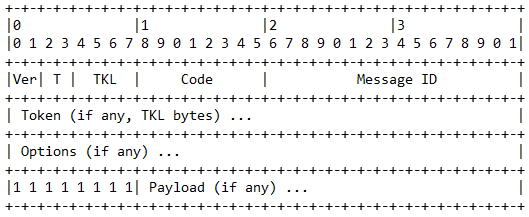
\includegraphics[width=0.8\textwidth]{MESSAGE_FORMAT}
	\caption{Formato da mensagem}
	\label{fig:message_format}
\end{figure}
%

\subsubsection{Cabeçalho}

Composto de: 
\begin{itemize}
	\item \textbf{Versão (Ver):} 2 bits do tipo  \textit{unsigned integer}. Valor 01, deve ser setado como 01, outros valores reservados. Caso receba mensagens com valor diferente, mensagem deve ser ignorada;
	\item \textbf{Tipo (T):} 2 bits do tipo  \textit{unsigned integer}, indica o tipo da mensagem, sendo: \textit{Confirmable} (0), \textit{Non-confirmable} (1), \textit{Acknowledgement} (2) ou \textit{Reset} (3);
	\item \textbf{Tamanho do \textit{Token}:} 4 bits do tipo  \textit{unsigned integer}. Indica o tamanho do campo \textit{token}, podendo ser de 0 a 8 bytes, valores de 0 a 8. Valores 9 a 15 reservados, caso a mensagem tenha algum desses valores, lidar como erro;
	\item \textbf{\textit{Code:}} 8 bits do tipo  \textit{unsigned integer}. Os 3 bits do tipo  \textit{unsigned integer} mais significantes são a classe, e outros 5 bits dão detalhes da mensagem, similar a resposta do protocolo HTTP. Veremos com detalhes no capítulos de pedidos e respostas, mas o eles são classificados conforme os 3 bits mais significativos:
	\begin{itemize}
		\item \textbf{0: } Indica pedido.
		\item \textbf{2: } Indica resposta bem sucedida.
		\item \textbf{4: } Resposta do cliente com erro.
		\item \textbf{5: } Resposta do servidor com erro.
		\item Código 0.00 indica mensagem vazia e demais códigos são reservados, outros códigos mais detalhados na imagem \ref{fig:cod_resp}. %%%%TABELA OU IMAGEM
		%%TABELA %%
	\end{itemize}
	\begin{figure}[!htb]
		\centering
		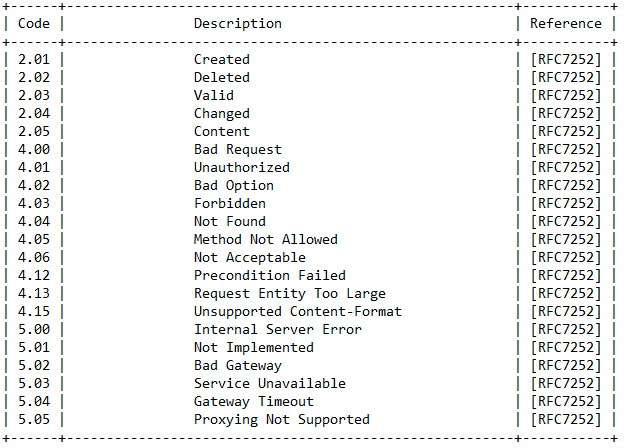
\includegraphics[width=0.8\textwidth]{CODE_RESPOSTAS}
		\caption{Códigos de resposta}
		\label{fig:cod_resp}
	\end{figure}
	\item \textit{\textbf{Message ID:}} 16 bits do tipo \textit{unsigned integer} em ordem, usado para detectar mensagens duplicadas e para combinar mensagens de ACK/\textit{Reset} com mensagens do tipo \textit{Confirmable}/\textit{Non-confirmable}.
\end{itemize}

\subsubsection {\textit{Token}}

Pode ser de tamanho entre 0 a 8 bytes, como determinado no campo TKL, é usado para relacionar pedidos e respostas.

\subsubsection {Opções}
\label{subsubsubsection{coap_option}}

O padrão CoAP define um número de opções máximas que pode ser incluído na mensagem. Cada opção deve incluir o número da opção, seguido do tamanho do valor da opção e por último o valor da opção. A imagem \ref{fig:opcoes_format} seguir demonstra como são formadas as opções. Abaixo estão suas definições:
\begin{figure}[!htb]
	\centering
	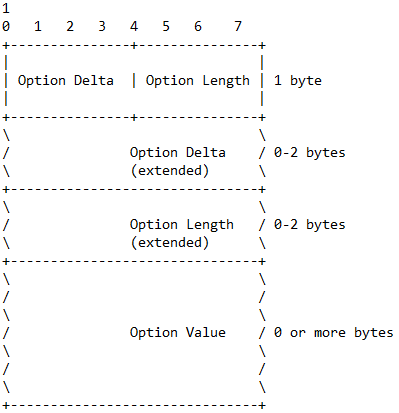
\includegraphics[width=0.8\textwidth]{OPTIONS}
	\caption{Formato Opções}
	\label{fig:opcoes_format}
\end{figure}

\begin{itemize}
	\item \textit{\textbf{Option Delta: }}4 bits do tipo \textit{unsigned integer}. Um valor entre 0 a 12 indica o valor do Delta da opção. Três valores são reservados.
	\begin{itemize}
		\item \textbf{13: }Um valor do tipo \textit{unsigned integer} de 8 bits segue o byte inicial e indica o \textit{Option Delta} menos 13.
		\item \textbf{14: }Um valor do tipo \textit{unsigned integer} de 16 bits segue o byte inicial e indica o \textit{Option Delta} menos 269.
		\item \textbf{15: }Reservado para \textit{Payload Marker}.
	\end{itemize}
	\item \textit{\textbf{Option Length: }} 4 bits do tipo \textit{unsigned integer}. Um valor entre 0 a 12  indicando o tamanho do valor da opção, em bytes. Três valores são reservados.
	\begin{itemize}
		\item \textbf{13: }Um valor do tipo \textit{unsigned integer} de 8 bits segue o byte inicial e indica o \textit{Option Length} menos 13.
		\item \textbf{14: }Um valor do tipo \textit{unsigned integer} de 16 bits segue o byte inicial e indica o \textit{Option Lenght} menos 269.
		\item \textbf{15: }Reservado para \textit{Payload Marker}.
	\end{itemize}
	\item \textit{\textbf{Option Value:}} O valor da opção não é definido diretamente, ele deve ser calculado utilizando o valor da opção e um delta. Sendo calculado da seguinte forma, o valor da opção atual é igual a soma do delta, o campo enviado na mensagem, mais o número da Opção anterior que deve ser armazenado no servidor. O valor inicial da opção anterior será zero. Além disso, o valor da opção segue os seguintes formatos:
	\begin{itemize}
		\item \textit{empty}: Uma sequência de bits de tamanho 0, indicando um valor vazio.
		\item \textit{opaque}: Uma sequência de bits cuja estrutura de dados não está definida.
		\item \textit{uint}: Um inteiro não negativo representado em ordem usando números de bytes dados. Deve ser definido e deve representar inteiros com o menor número de bytes possível.
		\item \textit{string}: Uma string codificada em UTF-8 na forma Net-Unicode \cite{rfc7252_CoAP}.	
	\end{itemize}
\end{itemize}
Possíveis valores de opção conforme tabela \ref{coap_opcoes}.
\begin{table}[!htb]
	\centering
	\caption{Opções CoAP}
	\label{coap_opcoes}
	\begin{tabular}{l|l|l}
		Number & Name           & Reference  \\ \hline
		0      & (Reserved)     & [RFC7252]  \\ \hline
		1      & If-Match       & [RFC7252]  \\ \hline
		3      & Uri-Host       & [RFC7252]  \\ \hline
		4      & ETag           & [RFC7252]  \\ \hline
		5      & If-None-Match  & [RFC7252]  \\ \hline
		7      & Uri-Port       & [RFC7252]  \\ \hline
		8      & Location-Path  & [RFC7252]  \\ \hline
		11     & Uri-Path       & [RFC7252]  \\ \hline
		12     & Content-Format & [RFC7252]  \\ \hline
		14     & Max-Age        & [RFC7252]  \\ \hline
		15     & Uri-Query      & [RFC7252]  \\ \hline
		17     & Accept         & [RFC7252]  \\ \hline
		20     & Location-Query & [RFC7252]  \\ \hline
		35     & Proxy-Uri      & [RFC7252]  \\ \hline
		39     & Proxy0Scheme   & [RFC7252]  \\ \hline
		60     & Size1          & [RFC7252]  \\ \hline
		128    & (Reserved)     & [RFC7252]  \\ \hline
		132    & (Reserved)     & [RFC7252]  \\ \hline
		136    & (Reserved)     & [RFC7252]  \\ \hline
		140    & (Reserved)     & [RFC7252] 
	\end{tabular}
\end{table}

\hfill \break
\hfill \break
\hfill \break
\hfill \break
\hfill \break
\hfill \break
\subsubsection {\textit{Payload}}

Deve ser indicado com um byte chamado \textit{Payload Marker}, de valor 0xFF, que indica o fim das opções e início do \textit{payload}. Terá o tamanho definido pelo final do pacote UDP, a partir do byte \textit{Payload Marker}. Caso não haja um \textit{Payload Marker}, o \textit{payload} deve ser lido como tamanho zero. Caso exista um \textit{Payload Marker} não seguido por um \textit{payload} de tamanho zero, tratar como erro.

\subsection{Confiabilidade}

A troca de mensagens entre nós de forma confiável é feita com o uso de mensagens Confimable. Esse tipo de mensagem sempre carrega um pedido ou uma resposta, a não ser que seja usada para \textit{Reset}, sendo uma mensagem vazia.
O servidor deve mandar um ACK em uma mensagem \textit{Confirmable} ou rejeitar a mensagem caso não possa processar, enviando uma mensagem de \textit{Reset} ou ignorando a mensagem. O ACK deve repetir o campo \textit{Message ID} da mensagem \textit{Confirmable} e carregar uma resposta ou ser vazia.  Caso ele envie o conteúdo da resposta no mesmo pacote do ACK, chamamos isso de Piggybacked response.
O cliente ou servidor enviarão a mensagem em intervalos crescentes, até receber um ACK, ou \textit{Reset}, ou ainda ficar sem tentativas de envio, como veremos a seguir.
A retransmissão é controlada através de dois parâmetros, que devem ser gerenciadas pelo dispositivo transmissor, para cada mensagem \textit{Confirmable}, um \textit{timeout} e um contador de retransmissões. Para cada retransmissão, o \textit{timeout} é dobrado, iniciando de um valor randômico entre ACK\_TIMEOUT e (ACK\_TIMEOUT x ACK\_RANDOM\_FACTOR), conforme tabela abaixo. O transmissor ainda pode desistir da mensagem caso a mensagem perca o propósito ou receba outros erros a serem tratados.
Mensagens não confiáveis podem ser utilizadas também, sendo útil em casos de uma mensagem que é transmitida regularmente e de mesmo conteúdo, utilizando o modo \textit{\textit{Non-confirmable}}.
Para manter o tráfego controlado, o padrão CoAP também limita o número máximo de iterações simultâneas para um valor configurável, NSTART.


\subsection{Correlação da mensagem e mensagens duplicadas}

As mensagens são relacionadas através do campo \textit{Message ID} com uma informação adicional do endpoint. O \textit{Message ID} é um valor de 16 bits do tipo \textit{unsigned integer}, gerado pelo transmissor. Esse \textit{Message ID} deve ser copiado na resposta em uma mensagem do tipo ACK ou \textit{Reset} pelo receptor. Além disso, o \textit{Message ID} não deve ser reutilizado, com o mesmo endpoint, dentro do tempo EXCHANGE\_LIFETIME, figura \ref{coap_parametro_deriv}.
O receptor pode coletar mais de uma mensagem \textit{Confirmable} com mesmo conteúdo, pode ser descoberto comparando a \textit{Message ID} e o nó fonte, múltiplas vezes dentro do EXCHANGE\_LIFETIME, ele deve enviar mensagens de ACK ou \textit{Reset} para todas as mensagens duplicadas recebidas, porém, só deve processar a mensagem uma vez.


\subsection{Tamanho da mensagem}

O padrão CoAP se beneficia de mensagens pequenas, facilitando tanto na criação da mensagem pelo embarcado, quanto para a rede, mas ele não estabelece um tamanho mínimo, apenas um tamanho máximo, porém uma mensagem maior que um pacote IP resulta em fragmentação da mensagem, portanto o padrão sugere que a mensagem seja menor que um pacote IP.

\subsection{Parâmetros de transmissão}

Os valores padrões utilizados para retransmissão seguem os valores da tabela \ref{coap_parametro_default}.

\begin{table}[!htb]
	\centering
	\caption{Parâmetros padrões CoAP}
	\label{coap_parametro_default}
	\begin{tabular}{l|l}
		\hline
		name                & default vale  \\ \hline
		ACK\_TIMEOUT        & 2 seconds     \\ \hline
		ACK\_RANDOM\_FACTOR & 1.5           \\ \hline
		MAX\_RETRANSMIT     & 4             \\ \hline
		NSTART              & 1             \\ \hline
		DEFAULT\_LEISURE    & 5 seconds     \\ \hline
		PROBING\_RATE       & 1 byte/second \\ \hline
	\end{tabular}
\end{table}

Ainda podemos calcular outros valores, derivados dos primeiros, que são utilizados no padrão, conforme podemos ver na tabela \ref{coap_parametro_deriv}. Para mais detalhes, consultar a RFC7252 \cite{rfc7252_CoAP}.

\begin{table}[!htb]
	\centering
	\footnotesize\setlength{\tabcolsep}{25pt}
	\caption{Parâmetros derivados CoAP}
	\label{coap_parametro_deriv}
	\begin{tabular}{l|r}
		\hline
		name                & \multicolumn{1}{l}{default value} \\ \hline
		MAX\_TRANSMIT\_SPAN & 45 s                               \\ \hline
		MAX\_TRANSMIT\_WAIT & 93 s                               \\ \hline
		MAX\_LATENCY        & 100 s                              \\ \hline
		PROCESSING\_DELAY   & 2s                                 \\ \hline
		MAX\_RTT            & 202 s                              \\ \hline
		EXCHANGE\_LIFETIME  & 247 s                              \\ \hline
		NON\_LIFETIME       & 145 s                              \\ \hline
	\end{tabular}
\end{table}


\subsection{Pedidos e respostas}


Um pedido CoAP consiste em, um método que será aplicado, o identificador do recurso, o \textit{payload}, um \textit{Internet media type}, se presente e um \textit{metadata} opcional sobre o pedido. É identificado no campo \textit{code} do \textit{header}. Ele pode ser do tipo GET, POST, PUT e DELETE, seguindo a denominação do padrão HTTP para facilitar o entendimento deste novo padrão, conforme veremos a seguir na tabela \ref{coap_code_method}. Eles são \textit{idempotents}, ou seja, pode se invocar múltiplas vezes com mesmo efeito, com exceção do POST porque a sua função é determinada dependendo do recurso alvo.
A resposta é identificada da mesma forma, no campo \textit{code} do \textit{header}, tabela \ref{coap_resposta_code}, e indica o resultado da tentativa de entender o pedido.
As mensagens de pedido e resposta são relacionadas através do \textit{token}, ao invés do \textit{Message ID} como é feito com mensagens \textit{Confirmable} ou \textit{Non-confirmable} e \textit{Acknowledgement} ou \textit{Reset}.

\begin{table}[!htb]
	\centering
	\caption{Métodos CoAP pedido (\textit{code} \textit{header})}
	\label{coap_code_method}
	\begin{tabular}{l|l|l}
		\hline
		Code & Name    & Reference     \\ \hline
		0.01 & GET     & {[}RFC7252{]} \\ \hline
		0.02 & POST    & {[}RFC7252{]} \\ \hline
		0.03 & PUT     & {[}RFC7252{]} \\ \hline
		0.04 & DELETE  & {[}RFC7252{]} \\ \hline
	\end{tabular}
\end{table}

\begin{table}[!htb]
	\centering
	\footnotesize\setlength{\tabcolsep}{25pt}
	\caption{Código de respostas (\textit{code} \textit{header})}
	\label{coap_resposta_code}
	\begin{tabular}{l|l|l}
		\hline
		Code & Description                & Reference     \\ \hline
		2.01 & Created                    & {[}RFC7252{]} \\ \hline
		2.02 & Deleted                    & {[}RFC7252{]} \\ \hline
		2.03 & Valid                      & {[}RFC7252{]} \\ \hline
		2.04 & Changed                    & {[}RFC7252{]} \\ \hline
		2.05 & Content                    & {[}RFC7252{]} \\ \hline
		4.00 & Bad Request                & {[}RFC7252{]} \\ \hline
		4.01 & Unauthorized               & {[}RFC7252{]} \\ \hline
		4.02 & Bad Option                 & {[}RFC7252{]} \\ \hline
		4.03 & Forbidden                  & {[}RFC7252{]} \\ \hline
		4.04 & Not Found                  & {[}RFC7252{]} \\ \hline
		4.05 & Method Not Allowed         & {[}RFC7252{]} \\ \hline
		4.06 & Not Acceptable             & {[}RFC7252{]} \\ \hline
		4.12 & Precondition Failed        & {[}RFC7252{]} \\ \hline
		4.13 & Request Entity Too Large   & {[}RFC7252{]} \\ \hline
		4.15 & Unsopported Content-Format & {[}RFC7252{]} \\ \hline
		5.00 & Internal Server Error      & {[}RFC7252{]} \\ \hline
		5.01 & Not Implemented            & {[}RFC7252{]} \\ \hline
		5.02 & Bad Gateway                & {[}RFC7252{]} \\ \hline
		5.03 & Service Unavailable        & {[}RFC7252{]} \\ \hline
		5.04 & Gateway Timeout            & {[}RFC7252{]} \\ \hline
		5.05 & Proxying Not Supported     & {[}RFC7252{]} \\ \hline
	\end{tabular}
\end{table}


\subsection{Métodos}

Os métodos aceitos serão citados abaixo, caso haja um pedido com método não reconhecido ou não suportado, deve ser gerada uma \textit{Piggybacked response} \ref{subsection:msg_piggybacked} do tipo 4.05, método não permitido.

\subsubsection {GET}

Solicita a informação sobre o recurso identificado na URI.  Tipo de mensagem \textit{Non-Confirmable}.

\subsubsection {POST}
\label{subsubsection:post}
A função do método é determinada pelo servidor de origem e depende do recurso alvo. Usualmente resulta na criação de um novo recurso ou atualização do recurso alvo já existente. Tipo de mensagem \textit{Confirmable}.

\subsubsection {PUT}

O método PUT solicita que o recurso identificado na URI seja criado ou atualizado. Tipo de mensagem \textit{Non-Confirmable}.

\subsubsection {DELETE}

Define que o recurso identificado pela URI seja excluído.

\section{ESP8266}

É um módulo, de tamanho reduzido e baixo custo. Além de, nas suas versões mais atuais, ter a facilidade de comunicação micro-USB para implementação de código. Ele pode também ser utilizado de forma integrada a outro sistema embarcado utilizando a comunicação UART, para implementar a função de comunicação com a internet.


Ele existe em diversas versões, mas todas com praticamente o mesmo funcionamento. Sua CPU é baseada em um IP Xtensa, da Cadence, levemente modificado pela empresa fabricante Espressif.
Alguns de seus recursos de hardware são:

\begin{itemize}
	\item Conectores GPIO, barramentos I2C, SPI, UART, entrada ADC, saída PWM e sensor interno de temperatura;
	\item CPU que opera em 80MHz, com possibilidade de operar em 160MHz;
	\item Arquitetura RISC de 32 bits;
	\item 32KBytes de RAM para instruções;
	\item 96KBytes de RAM para dados;
	\item 64KBytes de ROM para boot;
	\item O núcleo é baseado no IP Diamand Standard LX3 da Tensilica;
	\item Fabricado pela Espressif;
	\item VCC de 3,3V para operar.
\end{itemize}

E algumas características de funcionamento são:
\begin{itemize}	
	\item Engine integrada para criptografias WEP, TKIP, AES e WPA;
	\item Suporte aos protocolos 802.11 b/g/n;
	\item Wi-Fi Direct (P2P), soft-AP;
	
	\item Pilha de protocolo TCP/IP integrada com suporte a IPv4;
	\item Wi-Fi em frequência de 2.4GHz com suporte a WPA e WPA2;
	\item Potência de saída em +20dBm no modo 802.11b;
	
	\item Conversor ADC integrado com resolução de 10 bits;
	\item Suporte a uma variedade de antenas;
	\item Energia de consumo em modo sleep menor que 10uA;
	
	\item Tempo para sair de sleep e transmitir pacotes menor que 2ms;
	\item Potência de standby menor que 1.0mW;
	\item Pode operar em faixa de temperaturas de -40ºC a 125ºC.
	
\end{itemize}

A empresa desenvolvedora Espressif \cite{espressif_ref} disponibiliza um repositório no GitHub para facilitar o desenvolvimento para este microcontrolador, com alguns exemplos já desenvolvidos \cite{esp8266_site}.